\documentclass[a4paper,10pt]{article}
\usepackage{fullpage}
\usepackage{float}
\usepackage[english]{babel}
\usepackage{graphicx,subfig,wrapfig}
\usepackage{amsmath,amsfonts,amsthm,amssymb} 
\usepackage{fancyhdr,fancybox,color}
\usepackage{epstopdf}
\usepackage{enumerate}
\usepackage{multirow}
\usepackage[amssymb]{SIunits}             	% SI units package
\definecolor{MyBlue}{rgb}{0,0.3,0.6}      	
\usepackage[colorlinks=true,linkcolor=MyBlue,plainpages=false,citecolor=MyBlue,urlcolor=MyBlue]{hyperref}
\usepackage[all]{hypcap}   					%fixes the hyperref, such that links are anchored at the bottom of the images, not the top
\usepackage{tcolorbox}
\usepackage[url=false,
backend=bibtex,
style=authoryear-comp,
doi=true,
isbn=true,
backref=false,
dashed=false,
maxcitenames=2,
maxbibnames=99,
natbib=true]{biblatex}
\DeclareNameAlias{author}{last-first}
\renewbibmacro{in:}{}
\addbibresource{../_logosAndRef/references.bib}

\definecolor{mgray}{gray}{0.85}
\definecolor{mpurple}{HTML}{68236D}
\nonfrenchspacing

\begin{document} 
\thispagestyle{empty} % remove the page number on this page

\noindent Chair: Physics of Fluids Department

\begin{center}
  \begin{LARGE}
   Holey sheets: Bursting of liquid films
  \end{LARGE}
\end{center}

\noindent Ever watched a soap bubble burst? The same physics governs critical processes from COVID-19 transmission through respiratory droplets to agricultural spray efficiency—yet the mechanism triggering holes in micron-thick liquid sheets remains contested.

\begin{tcolorbox}[colback=mgray,colframe=mpurple,title=TL;DR]
  Micron-thick liquid sheets routinely develop holes despite Van der Waals forces only operating at nanometer scales—a paradox critical to understanding respiratory droplet transmission and spray technologies. This project investigates how submicron impurities (bubbles, oil droplets) trigger hole nucleation through local thinning effects. Using Basilisk C with CLSVOF interface tracking, you'll simulate radial drainage flows to map the double threshold for breakup: sufficient drainage rate and initial perturbation size. We will extend existing code to include thermal/chemical effects, perform systematic parameter sweeps, and develop scaling laws for hole formation. Ideal for students seeking hands-on CFD experience with immediate applications to aerosol physics and industrial atomization.
\end{tcolorbox}

\section*{Description}

When droplets encounter uniform airflow, they deform into bag-like structures that ultimately fragment through hole formation and growth. Classical theory attributes this breakup to Van der Waals forces operating at molecular scales ($\sim 10\,\text{nm}$), yet experiments routinely observe hole nucleation in sheets hundreds of times thicker. 
This project tests a novel hypothesis: submicron impurities (bubbles, oil droplets) trigger hole formation at micron scales through local thinning and curvature effects. 
Using direct numerical simulations with Coupled-Level-Set-Volume-of-Fluid (CLSVOF) methods in Basilisk C, we will map the parameter space governing impurity-driven breakup, establishing quantitative thresholds for hole opening versus healing. Our findings will refine predictive models for aerosol dynamics and spray technologies, with direct applications to disease transmission modeling and industrial atomization processes.

\section*{Deep dive}

To model the inflating bag formation, we use a simplified axially symmetric radial drainage model, imposing an outward velocity $u = \omega r$, where $\omega$ is the drainage rate, and $r$ is the radial distance (see figure \ref{fig:droplets2021}). This approach captures the essence of bag-like expansion that follows a free-fall like drainage while isolating the hole formation mechanism.
We found that, even when impurities initiate hole formation, the film can heal if the radial driving is weak. Conversely, holes grow and lead to sheet breakup if the imposed flow rate and initial shape distortion are large.

Moreover, smaller cavities consistently heal, whereas larger perturbations always open. Potential chemical or thermal inhomogeneities may further influence these dynamics, delaying hole nucleation. These findings reveal a double threshold for hole formation underlying the role of submicron impurities in droplet fragmentation-the driving should be strong enough, and the initial shape distortions should be large enough-refining existing models of droplet breakup and can guide design strategies in aerosol and spray processes.
Several open questions emerge: 

\begin{enumerate}
  \item How do specific impurities or surface agents affect hole formation thresholds? 
  \item Does local heating or cooling shift the balance between healing and opening?
  \item  Could non-Newtonian effects or external forcing alter these conclusions?
\end{enumerate}

Addressing these questions could refine droplet breakup models and guide future designs in aerosol and spray technologies—offering a rich avenue of study for a bachelor's or master's research project.

\begin{figure}
\centering
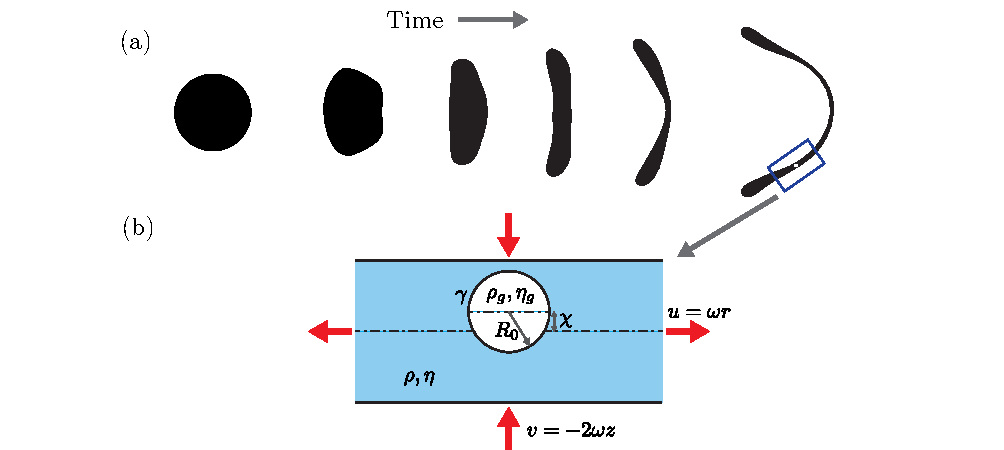
\includegraphics[width=\textwidth]{schematic_02.pdf}
\caption{(a) Droplet in uniform airflow deforms and expands into a bag-like structure. The impurities inside the sheets can prompt breakup when the thickness is of micron order. (b) To model that, bubbles as a defect are simulated inside a simplified two-dimensional liquid draining sheet.}
\label{fig:droplets2021}
\end{figure}

\section*{What you will do and what you will learn?}
In Computational Multiphase Physics Lab, we are looking for enthusiastic students to join our newly established project on bursting of sandwiched liquid films.

\begin{enumerate}
\item You will learn about film bursting, Taylor--Culick retractions, and viscous dissipation. 
\item You will work closely with experimentalists. 
\item You will learn about the Computational Fluid Dynamics (CFD) fundamentals, and use the free software program \href{http://basilisk.fr}{Basilisk C}.
\item You will have access to a read-to-use codebase (available on \href{https://github.com/comphy-lab/bubbleinSheet}{GitHub}).
\item You will learn how to do basic and advanced scientific data analysis.
\item As a part of the \href{https://comphy-lab.org}{CoMPhy lab}, you will learn and adapt open-source coding principles. 
\end{enumerate}

If you have any questions, feel free to contact \href{mailto:a.k.dixit@utwente.nl}{Ayush} (details below).
\begin{center}
\begin{tabular}{|l|l|l|}
\hline \textbf{Supervision} & \textbf{E-mail} & \textbf{Office} \\
\hline Ayush Dixit M.Sc. & \href{mailto:a.k.dixit@utwente.nl}{a.k.dixit@utwente.nl} & Meander 250 \\
\hline \multirow{2}{*}{Dr. Vatsal Sanjay} & \href{mailto:vatsal.sanjay@comphy-lab.org}{vatsal.sanjay@comphy-lab.org} & \multirow{2}{*}{Durham University} \\
& \href{mailto:vatsal.sanjay@durham.ac.uk}{vatsal.sanjay@durham.ac.uk} & \\
\hline Prof. Dr. Detlef Lohse F.R.S. & \href{mailto:d.lohse@utwente.nl}{d.lohse@utwente.nl} & Meander 261  \\
\hline
\end{tabular}
\end{center}

\printbibliography
\end{document}



